\newpage
\section{BIẾN CỐ HỢP VÀ QUY TẮC CỘNG XÁC SUẤT}
\subsection{TÓM TẮT LÝ THUYẾT}
\subsubsection{Biến cố hợp}
\begin{dn}
	{Cho hai biến cố $A$ và $B$. Biến cố \lq\lq$A$ hoặc $B$ xảy ra\rq\rq, kí hiệu là $A\cup B$ được gọi là \textbf{\textit{biến cố hợp}} của $A$ và $B$}
\end{dn}
\begin{note}
	{Biến cố $A \cup B$ xảy ra khi có ít nhất một trong hai biến cố $A$ và $B$ xảy ra. Tập hợp mô tả biến cố $A \cup B$ là hợp của hai tập hợp mô tả biến cố $A$ và biến cố $B$.}
\end{note}

\subsubsection{Quy tắc cộng xác suất}
\paragraph{Quy tắc cộng cho hai biến cố xung khắc}
\begin{dn}
	{Cho hai biến cố xung khắc $A$ và $B$. Khi đó $\mathrm{P}(A \cup B)=\mathrm{P}(A)+\mathrm{P}(B)$.}
\end{dn}

\paragraph{Quy tắc cộng cho hai biến cố bất kì}
\begin{dn}
	{Cho hai biến cố $A$ và $B$. Khi đó $\mathrm{P}(A \cup B)=\mathrm{P}(A)+\mathrm{P}(B)-\mathrm{P}(A B)$.}
\end{dn} 
\subsection{PHÂN LOẠI VÀ PHƯƠNG PHÁP GIẢI TOÁN}
\begin{dang}{Xác định biến cố hợp}
\end{dang}
\begin{vd}%[1T9B2-4]
	Một hộp chứa 5 viên bi xanh và 3 viên bi đỏ có cùng kích thước và khối lượng. Lấy ra ngẫu nhiên đồng thời 2 viên bi từ hộp. Gọi $A$ là biến cố \lq\lq Hai viên bi lấy ra đều có màu xanh\rq\rq, $B$ là biến cố \lq\lq Hai viên bi lấy ra đều có màu đỏ\rq\rq.
	\begin{enumerate}
		\item Có bao nhiêu kết quả thuận lợi cho biến cố $A$? Có bao nhiêu kết quả thuận lợi cho biến cố $B$?
		\item Hãy mô tả bằng lời biến cố $A \cup B$ và tính số kết quả thuận lợi cho biến cố $A \cup B$.
	\end{enumerate}
	\loigiai{
		\begin{enumerate}
			\item Số kết quả thuận lợi cho biến cố $A$ là $\mathrm{C}_5^2=10$. Số kết quả thuận lợi cho biến cố $B$ là $\mathrm{C}_3^2=3$.
			\item $A \cup B$ là biến cố \lq\lq Hai viên bi lấy ra có cùng màu\rq\rq. Số kết quả thuận lợi cho biến cố $A \cup B$ là $\mathrm{C}_5^2+\mathrm{C}_3^2=13$.
		\end{enumerate}
	}
\end{vd}
\begin{vd}%[1T9B2-2]
	Thực hiện hai thí nghiệm. Gọi $T_1$ và $T_2$ lần lượt là các biến cố \lq\lq Thí nghiệm thứ nhất thành công\rq\rq và \lq\lq Thí nghiệm thứ hai thành công\rq\rq. Hãy biểu diễn các biến cố sau theo hai biến cố $T_1$ và $T_2$.
	\begin{enumerate}
		\item $A$: \lq\lq Có ít nhất một trong hai thí nghiệm thành công\rq\rq.
		\item $B$: \lq\lq Có đúng một trong hai thí nghiệm thành công\rq\rq.
	\end{enumerate}
	\loigiai{
		\begin{enumerate}
			\item $A=T_1 \cup T_2$.
			\item $B=\overline{T_1} T_2 \cup T_1 \overline{T}_2$.
		\end{enumerate}
	}
\end{vd}
\begin{dang}{Quy tắc cộng cho hai biến cố xung khắc}
	Cho hai biến cố xung khắc $A$ và $B$. Khi đó $\mathrm{P}(A \cup B)=\mathrm{P}(A)+\mathrm{P}(B)$.
\end{dang}

\begin{vd}%[1D9H2-5]
	Cho $A$ và $B$ là hai biến cố độc lập và $\mathrm{P}(A)=0{,}5$; $\mathrm{P}(B)=0{,}4$.
	\begin{enumerate}
		\item Tính $\mathrm{P}(A\cap B)$.
		\item Tính $\mathrm{P}(A\cup B)$.
	\end{enumerate}
	\loigiai{
		\begin{enumerate}
			\item Vì $A$ và $B$ là hai biến cố độc lập nên
			$$\mathrm{P}(A\cap B)=\mathrm{P}(A)\cdot \mathrm{P}(B)=0{,}5\cdot 0{,}4=0{,}2.$$
			\item Ta có 
			$$\mathrm{P}(A\cup B)=\mathrm{P}(A)+\mathrm{P}(B)-\mathrm{P}(A\cap B)=0{,}5+0{,}4-0{,}2=0{,}7.$$
		\end{enumerate}
	}
\end{vd}
\begin{vd}%[1T9K2-4]
	Một đội tình nguyện gồm 9 học sinh khối 10 và 7 học sinh khối 11. Chọn ra ngẫu nhiên 3 người trong đội. Tính xác suất của biến cố \lq\lq Cả 3 người được chọn học cùng một khối\rq\rq.
	\loigiai{
		Gọi $A$ là biến cố \lq\lq Cả 3 học sinh được chọn đều thuộc khối 10 \rq\rq và $B$ là biến cố \lq\lq Cả 3 học sinh được chọn đều thuộc khối 11\rq\rq. Khi đó $A \cup B$ là biến cố \lq\lq Cả 3 người được chọn học cùng một khối\rq\rq. Do $A$ và $B$ là hai biến cố xung khắc nên $\mathrm{P}(A \cup B)=\mathrm{P}(A)+\mathrm{P}(B)$.\\
		Ta thấy $\mathrm{P}(A)=\dfrac{\mathrm{C}_9^3}{\mathrm{C}_{16}^3}$ và $\mathrm{P}(B)=\dfrac{\mathrm{C}_7^3}{\mathrm{C}_{16}^3}$, nên $\mathrm{P}(A \cup B)=\dfrac{\mathrm{C}_9^3+\mathrm{C}_7^3}{\mathrm{C}_{16}^3}=\dfrac{17}{80}$.
	}
\end{vd}
\begin{vd}%[1T9K2-4]
	Ở lúa, hạt gạo đục là tính trạng trội hoàn toàn so với hạt gạo trong. Cho cây lúa có hạt gạo đục thuần chủng thụ phấn với cây lúa có hạt gạo trong được $\mathrm{F}1$ toàn hạt gạo đục. Tiếp tục cho các cây lúa $\mathrm{F}1$ thụ phấn với nhau và thu được các hạt gạo mới. Lần lượt chọn ra ngẫu nhiên 2 hạt gạo mới, tính xác suất của biến cố \lq\lq Có đúng 1 hạt gạo đục trong 2 hạt gạo được lấy ra\rq\rq.
	\loigiai{
		Quy ước gene $\mathrm{A}$: hạt gạo đục và gene $\mathrm{a}$: hạt gạo trong. Ở thế hệ $\mathrm{F}2$, ba kiểu gene $\mathrm{AA},\mathrm{Aa}$, aa xuất hiện với tỉ lệ $1: 2: 1$ nên tỉ lệ hạt gạo đục so với hạt gạo trong là $3:1$.\\
		Gọi $A_1, A_2$ lần lượt là biến cố \lq\lq Hạt gạo lấy ra lần thứ nhất là hạt gạo đục\rq\rq\, và biến cố \lq\lq Hạt gạo lấy ra lần thứ hai là hạt gạo đục\rq\rq.\\
		Ta có $A_1$, $A_2$ là hai biến cố độc lập và $\mathrm{P}\left(A_1\right)=\mathrm{P}\left(A_2\right)=\dfrac{3}{4}$. Xác suất của biến cố \lq\lq Có đúng 1 hạt gạo đục trong 2 hạt gạo được lấy ra\rq\rq \,là\\
		$\mathrm{P}\left(A_1 \overline{A}_2 \cup \overline{A}_1 A_2\right)=\mathrm{P}\left(A_1 \overline{A}_2\right)+\mathrm{P}\left(\overline{A}_1 A_2\right)=\mathrm{P}\left(A_1\right) \mathrm{P}\left(\overline{A}_2\right)+\mathrm{P}\left(\overline{A}_1\right) \mathrm{P}\left(A_2\right)=2 \cdot \dfrac{3}{4}\cdot \dfrac{1}{4}=\dfrac{3}{8}$.
	}
\end{vd}
\begin{dang}{Quy tắc cộng cho hai biến cố bất kỳ}
	Cho hai biến cố $A$ và $B$. Khi đó $\mathrm{P}(A \cup B)=\mathrm{P}(A)+\mathrm{P}(B)-\mathrm{P}(A B)$.
\end{dang}
\begin{vd}%[1T9K2-4]
	Một hộp chứa $100$ tấm thẻ cùng loại được đánh số lần lượt từ 1 đến 100. Chọn ngẫu nhiên 1 thẻ từ hộp. Tính xác suất của biến cố \lq\lq Số ghi trên thẻ được chọn chia hết cho 3 hoặc 5\rq\rq.
	\loigiai{
		Gọi $A$ là biến cố \lq\lq Số ghi trên thẻ được chọn chia hết cho 3\rq\rq và $B$ là biến cố \lq\lq Số ghi trên thẻ được chọn chia hết cho 5\rq\rq.\\
		$A \cup B$ là biến cố \lq\lq Số ghi trên thẻ được chọn chia hết cho 3 hoặc 5\rq\rq.\\
		Từ 1 đến 100 có 33 số chia hết cho 3 nên $\mathrm{P}(A)=\dfrac{33}{100}=0,33$.\\
		Từ 1 đến 100 có 20 số chia hết cho 5 nên $\mathrm{P}(B)=\dfrac{20}{100}=0,2$.\\
		Một số chia hết cho cả 3 và 5 khi nó chia hết cho 15. Từ 1 đến 100 có 6 số chia hết cho 15 nên\\
		\centerline{$\mathrm{P}(A B)=\dfrac{6}{100}=0,06$}.\\
		Vậy $\mathrm{P}(A \cup B)=\mathrm{P}(A)+\mathrm{P}(B)-\mathrm{P}(A B)=0,33+0,2-0,06=0,47$.
	}
\end{vd}
\subsection{BÀI TẬP RÈN LUYỆN}
\ind{PHẦN I.} \inden{Câu trắc nghiệm nhiều phương án lựa chọn. Mỗi câu hỏi học sinh chỉ chọn một phương án.}\\
\setcounter{ex}{0}
\Opensolutionfile{ans}[ans/11T9-Bai1-TN]%--Đặt tên 11T9-Bai1-Dang1-TN
%C:\Users\hppp\Desktop\Toan\ChuyenDeGK-CK-cacTruong\1.SAULUOI2025\SpDuAn-A-Dot11\data\HKII\1-TL-TN-THPT-HuongHoa-QuangTri-HKII-NH24-25.tex
\begin{ex}[Trích đề HKII THPT 2024 - 2025 Hướng Hóa - Quảng Trị]%[1D9N2-1]%[Dự án đề kiểm tra Toán 11 HKII NH24-25- Phan Anh]%[THPT Hướng Hóa- Quảng Trị]
	Cho $A$ và $B$ là hai biến cố. Biến cố hợp của $A$ và $B$ có nghĩa là
	\choice
	{$A$ và $B$ không xảy ra}
	{$A$ và $B$ cùng xảy ra}
	{$A$ không xảy ra}
	{\True $A$ hoặc $B$ xảy ra}
	\loigiai{Biến cố hợp của $A$ và $B$ có nghĩa là $A$ hoặc $B$ xảy ra.}
\end{ex}

%C:\Users\hppp\Desktop\Toan\ChuyenDeGK-CK-cacTruong\1.SAULUOI2025\SpDuAn-A-Dot11\data\HKII\1-TN-DS-TLN-TL-THPT-CheLanVien-QuangTri-HKII-NH24-25.tex
\begin{ex}[Trích đề HKII THPT 2024 - 2025 Chế Lan Viên - Quảng Trị]%[1D9N2-1]%[Dự án đề kiểm tra Toán 11 HKII NH24-25- Xuan Vy Pham]%[THPT Chế Lan Vien - Quảng Trị]
	Cho hai biến cố $A$ và $B$. Nếu việc xảy ra hay không xảy ra của biến cố này không ảnh hưởng đến xác suất xảy ra của biến cố kia thì hai biến cố $A$ và $B$ được gọi là
	\choice
	{xung khắc với nhau}
	{\True độc lập với nhau}
	{biến cố đối của nhau}
	{không giao nhau}
	\loigiai{Cho hai biến cố $A$ và $B$. Nếu việc xảy ra hay không xảy ra của biến cố này không ảnh hưởng đến xác suất xảy ra của biến cố kia thì hai biến cố $A$ và $B$ được gọi là độc lập với nhau.
	}
\end{ex}

%C:\Users\hppp\Desktop\Toan\ChuyenDeGK-CK-cacTruong\1.SAULUOI2025\SpDuAn-A-Dot11\data\HKII\1-TN-DS-TLN-TL-THPT-CheLanVien-QuangTri-HKII-NH24-25.tex
\begin{ex}[Trích đề HKII 2024 - 2025 THPT Chế Lan Viên - Quảng Trị]%[1D9N2-4]%[Dự án đề kiểm tra Toán 11 HKII NH24-25- Xuan Vy Pham]%[THPT Chế Lan Vien - Quảng Trị]
	Hai xạ thủ bắn cung vào bia. Gọi $X_1$ và $X_2$ lần lượt là các biến cố \lq \lq Xạ thủ thứ nhất bắn trúng bia\rq \rq \, và \lq \lq Xạ thủ thứ hai bắn trúng bia\rq \rq. Gọi $A$ là biến cố \lq \lq Cả hai xạ thủ bắn trúng bia\rq \rq, hãy biểu diễn biến cố $A$ theo hai biến cố
	$X_1$ và $X_2$.
	\choice
	{$A=X_1 \cup X_2$}
	{\True $A=X_1 \cap X_2$}
	{$A=\overline{X_1} \cup X_2$}
	{$A=X_1 \cup \overline{X_2}$}
	\loigiai{Vì $A$ là biến cố \lq \lq Cả hai xạ thủ bắn trúng bia\rq \rq nên $A=X_1 \cap X_2$.
	}
\end{ex}

%C:\Users\hppp\Desktop\Toan\ChuyenDeGK-CK-cacTruong\1.SAULUOI2025\SpDuAn-A-Dot11\data\HKII\1-TN-DS-TLN-TL-THPT-CheLanVien-QuangTri-HKII-NH24-25.tex
\begin{ex}[Trích đề HKII 2024 - 2025 THPT Chế Lan Viên - Quảng Trị]%[1D9N2-4]%[Dự án đề kiểm tra Toán 11 HKII NH24-25- Xuan Vy Pham]%[THPT Chế Lan Vien - Quảng Trị]
	Trong một cuộc khảo sát về mức sống của người Hà Nội, người khảo sát chọn ngẫu nhiên một gia
	đình ở Hà Nội. Xét các biến cố sau:\\
	$T$: \lq \lq Gia đình có tivi \rq \rq;\\
	$M$: \lq \lq Gia đình có máy vi tính \rq \rq;\\
	$E$: \lq \lq Gia đình có ít nhất một trong hai thiết bị \rq \rq;\\
	Khẳng định nào sau đây đúng?
	\choice
	{$M=E \cap T$}
	{$E=M \cap T$}
	{\True $E=M \cup T$}
	{$T=E \cup M$}
	\loigiai{Ta có $E$: \lq \lq Gia đình có ít nhất một trong hai thiết bị \rq \rq nên $E=M \cup T$.
	}
\end{ex}

%C:\Users\hppp\Desktop\Toan\ChuyenDeGK-CK-cacTruong\1.SAULUOI2025\SpDuAn-A-Dot11\data\HKII\1-TN-DS-TLN-TL-THPT-NgoQuyen-DaNang-HKII-NH24-25.tex
\begin{ex}[Trích đề HKII 2024 - 2025 THPT Ngô Quyền - Đà Nẵng ]%[1D9N2-1]%[Dự án đề kiểm tra Toán khối 11 HKII NH24-25-Dot11-Khắc Thiên]%[THPT Ngô Quyền - Đà Nẵng]
	Cho hai biến cố $A$ và $B$. Nếu việc xảy ra hay không xảy ra của biến cố này không ảnh hưởng đến xác suất xảy ra của biến cố kia thì hai biến cố $A$ và $B$ được gọi là
	\choice
	{xung khắc với nhau}
	{biến cố đối của nhau}
	{\True độc lập với nhau}
	{không giao với nhau}
	\loigiai{Nếu việc xảy ra hay không xảy ra của biến cố này không ảnh hưởng đến xác suất xảy ra của biến cố kia thì hai biến cố $A$ và $B$ được gọi là độc lập với nhau.}
\end{ex}


%C:\Users\hppp\Desktop\Toan\ChuyenDeGK-CK-cacTruong\1.SAULUOI2025\SpDuAn-A-Dot11\data\HKII\1-TN-DS-TL-THPT-TranPhu-HCM-HKII-NH24-25.tex
\begin{ex}[Trích đề HKII 2024 - 2025 THPT Trần Phú - TPHCM] %[1D9N2-2]%[Đề thi HKII LỚP 11 THPT-TranPhu-TPHCM-NH24-25]%[Nguyễn Ngọc Huy Trường]
	Một hộp đựng $20$ tấm thẻ cùng loại được đánh số từ $1$ đến $20$. Rút ngẫu nhiên một tấm thẻ trong hộp. Gọi $A$ là biến cố \lq\lq Rút được tấm thẻ ghi số chẵn lớn hơn $9$\rq\rq; $B$ là biến cố \lq\lq Rút được tấm thẻ ghi số không nhỏ hơn $8$ và không lớn hơn $14$\rq\rq. Số phần tử của $A \cup B$ là
	\choice
	{$10$}
	{$12$}
	{\True $13$}
	{$11$}
	\loigiai{
		Ta có $A=\{10;11;12;\ldots;20\}$ và
		$B=\{8;9;10;11;12;13;14\}$. \\
		Suy ra $A\cup B=\{8;9;10;\ldots;20\}$. Do đó $n(A\cup B)=13$.
	}
\end{ex}
%C:\Users\hppp\Desktop\Toan\ChuyenDeGK-CK-cacTruong\1.SAULUOI2025\SpDuAn-A-Dot12\data\HKII\1-TN-DS-TL-N-TL-THPT-PhamVanDong-QuangNgai-HKII-NH24-25.tex
\begin{ex}[Trích đề HKII 2024 - 2025 THPT Phạm Văn Đồng - Quảng Ngãi]%[1D9N2-1]%[Dự án đề kiểm tra Toán 11 GHK2 NH24-25- Huỳnh Đức Vũ]%[THPT PHẠM VĂN ĐỒNG-QUẢNG NGÃI]
	Xét phép thử ngẫu nhiên với không gian mẫu $\Omega $ có hai biến cố $A$ và $B$ xung khắc. Mệnh đề nào sau đây là đúng?
	\choice
	{\True $ \mathrm{P}(A\cup B)=\mathrm{P}(A)+\mathrm{P}(B)$}
	{$\mathrm{P}(A)=1-\mathrm{P}(B)$}
	{$ \mathrm{P}(AB)=\mathrm{P}(A)+\mathrm{P}(B)$}
	{$ A\cap B=\Omega $}
	\loigiai{
		Với hai biến cố A và B cùng liên quan đến một phép thử và xung khắc với nhau, ta có
		$$\mathrm{P}(A\cup B)=\mathrm{P}(A)+\mathrm{P}(B).$$}
\end{ex}

%C:\Users\hppp\Desktop\Toan\ChuyenDeGK-CK-cacTruong\1.SAULUOI2025\SpDuAn-A-Dot12\data\HKII\1-TN-DS-TLN-TL-THPT-NgoGiaTu-DakLak-GHKII-NH23-24.tex
\begin{ex}[Trích đề HKII 2024 - 2025 THPT Ngô Gia Tự - Đắk Lắk]%[1D9N2-4]%[Dự án đề kiểm tra Toán 11 HKII NH24-25- Nguyễn Tấn Tài]%[THPT NGÔ GIA TỰ - Daklak]
	Cho $A$, $B$ là hai biến cố xung khắc. Đẳng thức nào sau đây đúng?
	\choice
	{\True $\mathrm{P}(A\cup B)=\mathrm{P}(A)+\mathrm{P}(B)$}
	{$\mathrm{P}(A\cup B)=\mathrm{P}(A)\cdot \mathrm{P}(B)$}
	{$\mathrm{P}(A\cap B)=\mathrm{P}(A)+\mathrm{P}(B)$}
	{$\mathrm{P}(A\cup B)=\mathrm{P}(A)-\mathrm{P}(B)$}
	\loigiai{
		Vì $A,B$ là hai biến cố xung khắc nên $A\cap B=\varnothing$, do đó
		\begin{eqnarray*}
			\mathrm{P}(A\cup B)&=&\mathrm{P}(A)+\mathrm{P}(B)-\mathrm{P}(A\cap B)\\
			&=&\mathrm{P}(A)+\mathrm{P}(B).
		\end{eqnarray*}
		Vậy đẳng thức đúng là $\mathrm{P}(A\cup B)=\mathrm{P}(A)+\mathrm{P}(B)$.
	}
\end{ex}

%C:\Users\hppp\Desktop\Toan\ChuyenDeGK-CK-cacTruong\1.SAULUOI2025\SpDuAn-A-Dot12\data\HKII\1-TN-DS-TLN-TL-THPT-LuongNgocQuyen-ThaiNguyen-HKII-NH24-25.tex
\begin{ex}[Trích đề HKII 2024 - 2025 THPT Lương Ngọc Quyến - Thái Nguyên]%[HKII-2024-2025, THPT Lương Ngọc Quyến, Thái Nguyên]%[Trần Văn Hùng]%[1D9N2-1]
	Cho $A$ và $B$ là hai biến cố xung khắc. Khẳng định nào sau đây là {\bf sai}.
	\choice
	{$\mathrm{P}(A\cup B)=\mathrm{P}(A)+\mathrm{P}(B)-\mathrm{P}(A\cap B)$}
	{$\mathrm{P}(A\cup B)=\mathrm{P}(A)+\mathrm{P}(B)$}
	{$\mathrm{P}(A\cap B)=0$}
	{\True $\mathrm{P}(A\cup B)=\mathrm{P}(A\cap B)$}
	\loigiai{
		Vì $A$ và $B$ là hai biến cố xung khắc nên
		\begin{itemize}
			\item $A\cap B=\varnothing\Rightarrow \mathrm{P}(A\cap B)=0$;
			\item $\mathrm{P}(A\cup B)=\mathrm{P}(A)+\mathrm{P}(B)-\mathrm{P}(A\cap B)=\mathrm{P}(A)+\mathrm{P}(B)$.
		\end{itemize}
	}
\end{ex}
%C:\Users\hppp\Desktop\Toan\ChuyenDeGK-CK-cacTruong\1.SAULUOI2025\SpDuAn-A-Dot9\data\GHKII\1-TN-DS-TLN-TL-THPT-NinhBinh-BacLieu-GHKII-NH24-25.tex
\begin{ex}[Trích đề HKII 2024 - 2025 THPT Ninh Bình - Bạc Liêu]%[1D9N2-4] %[Dự án đề kiểm tra Toán 11 GHKII NH24-25-Nguyễn Hữu Duy]%[THPT Ninh Bình-Bạc Liêu]
	Cho hai biến cố $A$ và $B$ với $\mathrm{P}(A)=0{,}3$, $\mathrm{P}(B)=0{,}4$ và $\mathrm{P}(A \cup B)=0{,}6$. Tính $\mathrm{P}(A\cap B)$.
	\choice
	{\True $0{,}1$}
	{$0{,}2$}
	{$0{,}3$}
	{$0{,}4$}
	\loigiai{
		$\mathrm{P}(A\cap B)=\mathrm{P}(A)+\mathrm{P}(B)-\mathrm{P}(A \cup B)=0{,}6-0{,}3+0{,}4-0{,}6=0{,}1$.
	}
\end{ex}

%C:\Users\hppp\Desktop\Toan\ChuyenDeGK-CK-cacTruong\1.SAULUOI2025\SpDuAn-A-Dot9\data\GHKII\1-TN-DS-TLN-TL-THPT-Edison-HaiPhong-GKII-NH24-25.tex
\begin{ex}[Trích đề HKII 2024 - 2025 THPT Edison - Hải Phòng]%[1D9H2-2]%[Dự án tex đề GHKII THPT Edison - Hải Phòng- 24-25][Nguyễn Hữu Đức]
	Khi gieo một con xúc sắc, xác suất để mặt chấm chẵn xuất hiện là bao nhiêu?  
	\choice
	{\True $0{,}5$}  
	{$0{,}4$}  
	{$0{,}3$}  
	{$0{,}2$}  
	\loigiai{  
		Một con xúc sắc có $6$ mặt, gồm các số $\{1, 2, 3, 4, 5, 6\}$. Các mặt chấm chẵn là $\{2, 4, 6\}$, tức có $3$ mặt thỏa điều kiện.\\
		Xác suất xuất hiện mặt chấm chẵn là
		\[
		\mathrm{P}= \dfrac{\text{số kết quả thuận lợi}}{\text{tổng số kết quả có thể}} = \dfrac{3}{6} = 0{,}5.
		\]
	}  
\end{ex}

%C:\Users\hppp\Desktop\Toan\ChuyenDeGK-CK-cacTruong\1.SAULUOI2025\SpDuAn-A-Dot9\data\GHKII\1-TN-DS-TLN-TL-THPT-HauNghia-LongAn-GHKII-NH24-25.tex
\begin{ex}[Trích đề HKII 2024 - 2025 THPT Hậu Nghĩa - Long An]%[1D9H2-4]%[Dự án đề kiểm tra Toán 11 GHKII NH24-25 - Đợt 9 - Thành Đức Trung]%[THPT Hậu Nghĩa - Long An]
	Cho $A$, $B$ là hai biến cố độc lập, biết $\mathrm{P}(B)=0{,}5$, $\mathrm{P}(A\cup B) = 0{,}7$. Xác suất của biến cố $A$ là 
	\choice
	{$\mathrm{P}(A) = 0{,}3$}
	{\True $\mathrm{P}(A) = 0{,}4$}
	{$\mathrm{P}(A) = 0{,}7$}
	{$\mathrm{P}(A) = 0{,}5$}
	\loigiai
	{
		Do $A$, $B$ là hai biến cố độc lập nên
		$$\mathrm{P}(A\cup B) = \mathrm{P}(A) + \mathrm{P}(B) - \mathrm{P}(AB) = \mathrm{P}(A) + \mathrm{P}(B) - \mathrm{P}(A)\cdot \mathrm{P}(B).$$
		Kết hợp với $\mathrm{P}(B)=0{,}5$, $\mathrm{P}(A\cup B) = 0{,}7$ ta thu được 
		$$
		0{,}7 = 0{,}5 + \mathrm{P}(A) - 0{,}5 \mathrm{P}(A) \Leftrightarrow \mathrm{P}(A) = 0{,}4.
		$$
	}
\end{ex}

%C:\Users\hppp\Desktop\Toan\ChuyenDeGK-CK-cacTruong\1.SAULUOI2025\SpDuAn-A-Dot9\data\GHKII\1-TN-DS-TLN-TL-THPT-HauNghia-LongAn-GHKII-NH24-25.tex
\begin{ex}[Trích đề HKII 2024 - 2025 THPT Hậu Nghĩa - Long An]%[1D9N2-4]%[Dự án đề kiểm tra Toán 11 GHKII NH24-25 - Đợt 9 - Thành Đức Trung]%[THPT Hậu Nghĩa - Long An]
	Cho $A$, $B$ là hai biến cố độc lập. Khẳng định nào sau đây là đúng?
	\choice
	{$\mathrm{P}(A\cup B) = \mathrm{P}(A) + \mathrm{P}(B) + \mathrm{P}(AB)$}
	{$\mathrm{P}(AB) = \mathrm{P}(A)-\mathrm{P}(B)$}
	{\True $\mathrm{P}(AB) = \mathrm{P}(A) \cdot \mathrm{P}(B)$}
	{$\mathrm{P}(A\cup B) = \mathrm{P}(A) + \mathrm{P}(B)$}
	\loigiai
	{
		Do $A$, $B$ là hai biến cố độc lập nên $\mathrm{P}(AB) = \mathrm{P}(A) \cdot \mathrm{P}(B)$.
	}
\end{ex}

%C:\Users\hppp\Desktop\Toan\ChuyenDeGK-CK-cacTruong\1.SAULUOI2025\SpDuAn-A-Dot9\data\GHKII\1-TN-DS-TLN-TL-THPT-HoaHoi-BRVT-GHKII-NH24-25.tex
\begin{ex}[Trích đề HKII 2024 - 2025 THPT Hòa Hội - Tỉnh Bà Rịa Vũng Tàu]%[1D9N2-1]%[Dự án đề KT Toán khối 11 GKII NH24-25-Phạm Hoàng Đăng]%[THPT Hòa Hội - Tỉnh Bà Rịa Vũng Tàu]
	Gieo ngẫu nhiên một xúc xắc cân đối và đồng chất một lần. Xét biến cố $A$: \lq\lq Số chấm xuất hiện là số chia hết cho $2$\rq\rq\ và biến cố $B$: \lq\lq Số chấm xuất hiện là số chia hết cho $5$\rq\rq. Giá trị của $\mathrm{P}(A\cup B)$ là bao nhiêu?
	\choice
	{$\dfrac{1}{6}$}
	{$\dfrac{1}{2}$}
	{\True $\dfrac{2}{3}$}
	{$\dfrac{1}{3}$}
	\loigiai{
		Ta có $n(\Omega)=6$, $n(A)=3$, $n(B)=1$.\\ 
		Do $A\cap B=\varnothing$ nên $\mathrm{P}(A\cup B)=\mathrm{P}(A)+\mathrm{P}(B)=\dfrac{3}{6}+\dfrac{1}{6}=\dfrac{2}{3}$.
	}
\end{ex}

%C:\Users\hppp\Desktop\Toan\ChuyenDeGK-CK-cacTruong\1.SAULUOI2025\SpDuAn-A-Dot9\data\GHKII\1-TN-DS-TLN-TL-THPT-HoaHoi-BRVT-GHKII-NH24-25.tex
\begin{ex}[Trích đề HKII 2024 - 2025 THPT Hòa Hội - Tỉnh Bà Rịa Vũng Tàu]%[1D9N2-1]%[Dự án đề KT Toán khối 11 GKII NH24-25-Phạm Hoàng Đăng]%[THPT Hòa Hội - Tỉnh Bà Rịa Vũng Tàu]
	Cho hai biến cố $A$ và $B$. Khẳng định nào sau đây là đúng?
	\choice
	{$\mathrm{P}(A\cup B)=\mathrm{P}(A)+\mathrm{P}(B)$}
	{$\mathrm{P}(A\cup B)=\mathrm{P}(A) \cdot \mathrm{P}(B)$}
	{$\mathrm{P}(A\cup B)=\mathrm{P}(A)+\mathrm{P}(B)+\mathrm{P}(A\cap B)$}
	{\True $\mathrm{P}(A\cap B)=\mathrm{P}(A)+\mathrm{P}(B)-\mathrm{P}(A\cup B)$}
	\loigiai{
		$\mathrm{P}(A\cap B)=\mathrm{P}(A)+\mathrm{P}(B)-\mathrm{P}(A\cup B)$
	}
\end{ex}
\begin{ex}[Trích đề HKII 2024 - 2025 THPT Ngô Gia Tự - Đắk Lắk]%[1D9H2-4]%[Dự án đề kiểm tra Toán 11 HKII NH24-25- Nguyễn Tấn Tài]%[THPT NGÔ GIA TỰ - Daklak]
	Cho $A$, $B$ là hai biến cố xung khắc. Biết $\mathrm{P}(A)=\dfrac{1}{5}$, $\mathrm{P}(A\cup B)=\dfrac{1}{2}$. Tính $\mathrm{P}(B)$.
	\choice
	{$\dfrac{3}{5}$}
	{$\dfrac{8}{15}$}
	{$\dfrac{1}{15}$}
	{\True $\dfrac{3}{10}$}
	\loigiai{
		Vì $A,B$ là hai biến cố xung khắc nên
		\begin{eqnarray*}
			&&\mathrm{P}(A\cup B)=\mathrm{P}(A)+\mathrm{P}(B)\\
			&\Leftrightarrow&\dfrac{1}{2}=\dfrac{1}{5}+\mathrm{P}(B)\\
			&\Leftrightarrow&\mathrm{P}(B)=\dfrac{1}{2}-\dfrac{1}{5}\\
			&\Leftrightarrow&\mathrm{P}(B)=\dfrac{3}{10}.
		\end{eqnarray*}
		Vậy $\mathrm{P}(B)=\dfrac{3}{10}$.
	}
\end{ex}

%C:\Users\hppp\Desktop\Toan\ChuyenDeGK-CK-cacTruong\1.SAULUOI2025\SpDuAn-A-Dot11\data\HKII\1-TN-DS-TLN-TL-SGD-NamDinh-HKII-NH24-25.tex
\begin{ex}[Trích đề HKII 2024 - 2025 Sở Giáo dục Nam Định]%[1D9H2-2]%[1-TN-DS-TLN-TL-THPT-SGD-NamDinh-HKII-NH24-25]%[Nguyễn Văn Sang]
	Gieo ngẫu nhiên một con xúc xắc cân đối, đồng chất hai lần. Gọi $A$ là biến cố ``Số chấm xuất hiện trong hai lần gieo giống nhau'', B là biến cố ``Trong hai lần gieo có ít nhất một lần xuất hiện mặt $6$ chấm''. Số phần tử của biến cố $C = A \cup B$ là
	\choice
	{$18$}
	{$17$}
	{\True $16$}
	{$1$}
	\loigiai{
		Gọi $\Omega$ là không gian mẫu của phép thử gieo ngẫu nhiên một con xúc xắc cân đối, đồng chất hai lần. \\
		Mỗi phần tử của không gian mẫu có dạng $(i, j)$ với $i, j \in \{1, 2, 3, 4, 5, 6\}$.\\
		Số phần tử của không gian mẫu là $n(\Omega) = 6\cdot 6 = 36$. \\
		$A$ là biến cố ``Số chấm xuất hiện trong hai lần gieo giống nhau''.\\
		Các kết quả thuận lợi cho biến cố A là $A = \left\{(1, 1), (2, 2), (3, 3), (4, 4), (5, 5), (6, 6)\right\}$.\\
		Số phần tử của biến cố $A$ là $n(A) = 6$. \\
		$B$ là biến cố ``Trong hai lần gieo có ít nhất một lần xuất hiện mặt $6$ chấm''.\\
		Các kết quả thuận lợi cho biến cố $B$ là $$B = \left\{(1, 6), (2, 6), (3, 6), (4, 6), (5, 6), (6, 1), (6, 2), (6, 3), (6, 4), (6, 5), (6, 6)\right\}.$$
		Số phần tử của biến cố $B$ là $n(B) = 11$. \\
		Biến cố $C = A \cup B$ là biến cố hợp của A và B. \\
		Ta có $A \cap B$ là biến cố ``Số chấm xuất hiện trong hai lần gieo giống nhau và có ít nhất một lần xuất hiện mặt $6$ chấm''.\\
		Suy ra $A \cap B = \left\{(6, 6)\right\}$. Do đó $n(A \cap B) = 1$. \\
		Số phần tử của biến cố C là
		$$n(C) = n(A \cup B) = n(A) + n(B) - n(A \cap B) = 6 + 11 - 1 = 16.$$
	}
\end{ex}

%C:\Users\hppp\Desktop\Toan\ChuyenDeGK-CK-cacTruong\1.SAULUOI2025\SpDuAn-A-Dot11\data\HKII\1-TN-DS-TLN-TL-THPT-NgoGiaTu-PhuYen-HKII-NH24-25.tex
\begin{ex}[Trích đề HKII 2024 - 2025 THPT Ngô Gia Tự - Phú Yên]%[1D9H2-2]%[Dự án đề kiểm tra Toán 11 HKII NH24-25- Thầy Hóa]%[THPT - Ngô Gia Tự - Phú Yên]
	Một hộp đựng $20$ tấm thẻ cùng loại được đánh số từ $1$ đến $20$. Rút ngẫu nhiên một tấm thẻ trong hộp. Gọi $A$ là biến cố ``Rút được tấm thẻ ghi số chẵn lớn hơn $9$''; $B$ là biến cố ``Rút được tấm thẻ ghi số không nhỏ hơn $8$ và không lớn hơn $15$''. Số phần tử của $A\cup B$ là
	\choice
	{\True $11$}
	{$12$}
	{$10$}
	{$13$}
	\loigiai{
		Ta có $\begin{aligned}[t]
			A&=\{10;12;14;16;18;20\}\Rightarrow n(A)=6;\\
			B&=\{8;9;10;11;12;13;14;15\}\Rightarrow n(B)=8.
		\end{aligned}$\\
		Suy ra $A\cap B=\{10;12;14\}\Rightarrow n\left(A\cap B\right)=3$.\\
		Lại có $n\left(A\cup B\right)=n(A)+n(B)-n\left(A\cap B\right)$ nên
		\[n\left(A\cup B\right)=6+8-3=11. \]
	}
\end{ex}

%C:\Users\hppp\Desktop\Toan\ChuyenDeGK-CK-cacTruong\1.SAULUOI2025\SpDuAn-A-Dot11\data\HKII\1-TN-DS-TLN-TL-THPT-PhamPhuThu-DaNang-HKII-NH24-25.tex
\begin{ex}[Trích đề HKII 2024 - 2025 THPT Phạm Phú Thứ - Đà Nẵng]%[1D9H2-4]%[Kiểm tra CKII 24-25-Phạm Phú Thứ-Nguyễn Thanh Phong]%[Đà Nẵng]
Một hộp có $5$ viên bi màu đen, $4$ viên bi màu trắng. Chọn ngẫu nhiên $2$ viên bi từ chiếc hộp đó. Tìm xác suất để chọn được $2$ viên bi cùng màu.
		\choice
		{$\dfrac{1}{4}$}
		{\True $\dfrac{4}{9}$}
		{$\dfrac{1}{9}$}
		{$\dfrac{5}{4}$}
		\loigiai{
			Chọn ngẫu nhiên $2$ viên bi từ chiếc hộp, khi đó số phần tử của không gian mẫu là $n\left(\Omega\right)=\mathrm{C}_9^2$.\\ 
			Gọi $A$ là biến cố: \lq\lq Lấy được $2$ viên bi màu trắng\rq\rq, khi đó số kết quả thuận lợi là $\mathrm{C}_4^2$.\\		
			Suy ra $\mathrm{P}(A)=\dfrac{\mathrm{C}_4^2}{\mathrm{C}_9^2}=\dfrac{1}{6}$.\\
			Gọi $B$ là biến cố: \lq\lq Lấy được $2$ viên bi màu đen\rq\rq, khi đó số kết quả thuận lợi là $\mathrm{C}_5^2$.\\		 
			Suy ra $\mathrm{P}(B)=\dfrac{\mathrm{C}_5^2}{\mathrm{C}_9^2}=\dfrac{5}{18}$.\\
			Gọi $C$ là biến cố: \lq\lq Lấy được $2$ viên bi cùng màu\rq\rq.\\
			Ta có $C=A\cup B$ và $A$, $B$ là hai biến cố xung khắc.\\
			Vì vậy $\mathrm{P}(C)=\mathrm{P}(A)+\mathrm{P}(B)=\dfrac{4}{9}$.
		}
\end{ex}

%C:\Users\hppp\Desktop\Toan\ChuyenDeGK-CK-cacTruong\1.SAULUOI2025\SpDuAn-A-Dot11\data\HKII\1-TN-DS-TLN-TL-THPT-QueSon-QuangNam-HKII-NH24-25.tex
\begin{ex}[Trích đề HKII 2024 - 2025 THPT Quế Sơn - Quảng Nam]%[Đề kiểm tra HK2 lớp 11 THPT Quế Sơn-Quảng Nam 2024-2025]%[Nguyễn Tấn Linh]%[1D9H2-2]
	Gieo ngẫu nhiên một con xúc xắc cân đối, đồng chất một lần. Xét các biến cố ngẫu nhiên $A$: \lq\lq Mặt xuất hiện của xúc xắc có số chấm là số chẵn\rq\rq; $B$: \lq\lq Mặt xuất hiện của xúc xắc có số chấm là số chia hết cho $3$\rq\rq. Số phần tử của tập hợp $A \cup B$ là
	\choice
	{$2$}
	{$5$}
	{$3$}
	{\True $4$}
	\loigiai{
		Ta có $A = \{2; 4; 6\}$, $B = \{3; 6\}$.\\
		Suy ra $A \cup B = \{2; 3; 4; 6\}$.\\
		Vậy số phần tử của tập hợp $A \cup B$ là $4$.
	}
\end{ex}

\Closesolutionfile{ans}

\ind{PHẦN II.} \inden{Câu trắc nghiệm đúng sai. Trong mỗi ý a), b), c), d) ở mỗi câu, học sinh chọn đúng hoặc sai.}\\
\setcounter{ex}{0}
%C:\Users\hppp\Desktop\Toan\ChuyenDeGK-CK-cacTruong\1.SAULUOI2025\SpDuAn-A-Dot12\data\HKII\1-TN-DS-TLN-TL-THPT-NgoGiaTu-DakLak-GHKII-NH23-24.tex
\begin{ex}[Trích đề HKII 2024 - 2025 THPT Ngô Gia Tự - Daklak]%[1D9H2-3]%[Dự án đề kiểm tra Toán 11 HKII NH24-25- Nguyễn Tấn Tài]%[THPT NGÔ GIA TỰ - Daklak]
	Một hộp đựng $100$ tấm thẻ cùng loại được đánh số từ $1$ đến $100$. Rút ngẫu nhiên một tấm thẻ và quan sát số ghi trên thẻ.\\
	Gọi $A$ là biến cố \lq\lq Số ghi trên thẻ chia hết cho $3$ \rq\rq, $B$ là biến cố \lq\lq Số ghi trên thẻ chia hết cho $5$\rq\rq.
	\choiceTF
	{$\mathrm{P}(A)=\dfrac{31}{100}$ }
	{\True $\mathrm{P}(A\cap B)=\dfrac{3}{50}$ }
	{$A$ và $B$ xung khắc }
	{\True $\mathrm{P}(A\cup B)=\dfrac{47}{100}$ }
	\loigiai{
		\begin{itemchoice}
			\itemch Tổng số thẻ là $100$ nên $n\left( \Omega\right)=100$.\\
			Số thẻ chia hết cho $3$ là $\left\lfloor \dfrac{100}{3}\right\rfloor=33$ thẻ nên  $n(A)=33$.\\
			$\Rightarrow \mathrm{P}(A)=\dfrac{33}{100}$.
			\itemch Số thẻ chia hết cho cả $3$ và $5$ (hay chia hết cho $15$) là $\left\lfloor \dfrac{100}{15}\right\rfloor=6$ thẻ nên $n(A\cap B)=6$.\\
			$\Rightarrow \mathrm{P}(A\cap B)=\dfrac{6}{100}=\dfrac{3}{50}$.
			\itemch Vì $\mathrm{P}(A\cap B)=\dfrac{3}{50}\ne0$ nên $A$ và $B$ không xung khắc.
			\itemch Ta có\\
			Số thẻ chia hết cho $5$ là $\left\lfloor \dfrac{100}{5}\right\rfloor=20$ thẻ nên  $n(B)=20$.\\
			$\Rightarrow \mathrm{P}(B)=\dfrac{20}{100}$.\\
			$\mathrm{P}(A\cup B)=\mathrm{P}(A)+\mathrm{P}(B)-\mathrm{P}(A\cap B)=\dfrac{33}{100}+\dfrac{20}{100}-\dfrac{6}{100}=\dfrac{47}{100}$.
		\end{itemchoice}
	}
\end{ex}

%C:\Users\hppp\Desktop\Toan\ChuyenDeGK-CK-cacTruong\1.SAULUOI2025\SpDuAn-A-Dot11\data\HKII\1-TN-DS-TLN-TL-SGD-NamDinh-HKII-NH24-25.tex
\begin{ex}[Trích đề HKII 2024 - 2025 Sở Giáo dục Nam Định]%[1D9H2-3]%[1-TN-DS-TLN-TL-THPT-SGD-NamDinh-HKII-NH24-25]%[Nguyễn Văn Sang]
	Một hộp đựng $25$ tấm thẻ được đánh số từ $1$ đến $25$, hai tấm thẻ khác nhau đánh hai số khác nhau. Lấy ngẫu nhiên một tấm thẻ từ hộp, gọi $A$ là biến cố ``Số ghi trên thẻ chia hết cho $3$'', $B$ là biến cố ``Số ghi trên thẻ chia hết cho $10$''.
	\choiceTF
	{\True $\mathrm{P}(A) = \dfrac{8}{25}$}
	{ $\mathrm{P}(B) = \dfrac{3}{25}$}
	{\True $A$ và $B$ xung khắc}
	{\True $\mathrm{P}(A \cup B) = \dfrac{2}{5}$}
	\loigiai{
		Không gian mẫu $\Omega$ là tập hợp các số nguyên từ $1$ đến $25$, ta có $n(\Omega) = 25$.
		\begin{itemchoice}
			\itemch  Gọi $A$ là biến cố ``Số ghi trên thẻ chia hết cho $3$''.\\
			Các kết quả thuận lợi cho biến cố $A$ là $A = \{3, 6, 9, 12, 15, 18, 21, 24\}$.\\
			Số phần tử của $A$ là $n(A) = 8$.\\
			Xác suất của biến cố $A$ là $\mathrm{P}(A) = \dfrac{n(A)}{n(\Omega)} = \dfrac{8}{25}$.
			\itemch  Gọi $B$ là biến cố ``Số ghi trên thẻ chia hết cho $10$''.\\
			Các kết quả thuận lợi cho biến cố $B$ là $B = \{10, 20\}$.\\
			Số phần tử của $B$ là $n(B) = 2$.\\
			Xác suất của biến cố $B$ là $\mathrm{P}(B) = \dfrac{n(B)}{n(\Omega)} = \dfrac{2}{25}$.
			\itemch  Ta có $A \cap B$ là biến cố ``Số ghi trên thẻ chia hết cho cả $3$ và $10$'', tức là chia hết cho $30$. Vì không có số nào trong tập từ $1$ đến $25$ chia hết cho $30$ nên $A \cap B = \varnothing$.\\
			Do đó, $A$ và $B$ là hai biến cố xung khắc.
			\itemch Vì $A$ và $B$ là hai biến cố xung khắc, ta có công thức cộng xác suất\\
			$$\mathrm{P}(A \cup B) = \mathrm{P}(A) + \mathrm{P}(B) = \dfrac{8}{25} + \dfrac{2}{25} = \dfrac{2}{5}.$$
		\end{itemchoice}
	}
\end{ex}

%C:\Users\hppp\Desktop\Toan\ChuyenDeGK-CK-cacTruong\1.SAULUOI2025\SpDuAn-A-Dot11\data\HKII\1-TN-DS-TLN-TL-THPT-QueSon-QuangNam-HKII-NH24-25.tex
\begin{ex}[Trích đề HKII 2024 - 2025 THPT Quế Sơn - Quảng Nam]%[Đề kiểm tra HK2 lớp 11 THPT Quế Sơn-Quảng Nam 2024-2025]%[Nguyễn Tấn Linh]%[1D9H2-3]
	Gieo một con xúc xắc cân đối, đồng chất liên tiếp hai lần. Xét các biến cố sau:
	\begin{itemize}
		\item $A$: \lq\lq Số chấm xuất hiện trong hai lần gieo đều là số chẵn\rq\rq;
		\item $B$: \lq\lq Số chấm xuất hiện trong hai lần gieo gồm một số chẵn và một số lẻ\rq\rq;
		\item $C$: \lq\lq Tích số chấm xuất hiện trong hai lần gieo là số chẵn\rq\rq.
	\end{itemize}
	\choiceTF
	{\True Biến cố $C$ là hợp của hai biến cố $A$ và $B$}
	{\True $\mathrm{P}(C) = \mathrm{P}(A) + \mathrm{P}(B)$}
	{Xác suất của biến cố $A$ là $\dfrac{1}{6}$}
	{\True $\mathrm{P}(AB) = 0$}
	\loigiai{
		\begin{itemchoice}
			\itemch Tích số chấm xuất hiện trong hai lần gieo là số chẵn có hai trường hợp là
			\begin{itemize}
				\item Hai lần gieo đều là số chẵn;
				\item Hai lần gieo có một số chẵn và một số lẻ.
			\end{itemize}    
			Suy ra biến cố $C$ là hợp của hai biến cố $A$ và $B$.
			\itemch Vì $A$ và $B$ là hai biến cố xung khắc nên nên $\mathrm{P}(C)=\mathrm{P}(A\cup B) = \mathrm{P}(A) + \mathrm{P}(B)$.
			\itemch Ta có $n(\Omega)=6\cdot 6=36$.\\
			Xác suất của biến cố $A$ là $\mathrm{P}(A)=\dfrac{n(A)}{n(\Omega)}=\dfrac{3\cdot 3}{36}=\dfrac{1}{4}$.
			\itemch Vì hai biến cố $A$ và $B$ xung khắc nên $\mathrm{P}(AB)=0$.
		\end{itemchoice}	
	}
\end{ex}

%C:\Users\hppp\Desktop\Toan\ChuyenDeGK-CK-cacTruong\1.SAULUOI2025\SpDuAn-A-Dot11\data\HKII\1-TN-DS-TLN-THPT-LuongTheVinh-HaNoi-HKII-N24-25.tex
\begin{ex}[Trích đề HKII 2024 - 2025 THPT Lương Thế Vinh - Hà Nội]%[1D9H2-3]%[Dự án tex đề HKII THPT Lương Thế Vinh - Hà Nội- 24-25]%[Quan Ón]
	Một hộp chứa $21$ tấm thẻ cùng loại được đánh số từ $1$ đến $21$. Chọn ra ngẫu nhiên $1$ thẻ từ hộp. Gọi $A$ là biến cố \lq\lq Số ghi trên thẻ được chọn chia hết cho $2$\rq\rq, $B$ là biến cố \lq\lq Số ghi trên thẻ được chọn chia hết cho $3$\rq\rq.
	\choiceTF
	{\True $\mathrm{P}(A)=\dfrac{10}{21}$ và $\mathrm{P}(B)=\dfrac{1}{3}$}
	{Hai biến cố $A$ và $B$ xung khắc}
	{\True $\mathrm{P}(AB)=\dfrac{1}{7}$}
	{\True Hai biến cố $A$ và $B$ không độc lập}
	\loigiai{
		Ta có $\Omega = \{1;2;3;\dots;21\}\Rightarrow n(\Omega) = 21$.\\
		$A = \{2;4;6;\dots;20\} \Rightarrow n(A) = \dfrac{20-2}{2} + 1 = 10$.\\
		$B = \{3;6;9;\dots;21\} \Rightarrow n(B) = \dfrac{21-3}{3} + 1 = 7$.
		\begin{itemchoice}
			\itemch \textbf{Đúng}. Xác suất của biến cố $A$ là $\mathrm{P}(A) = \dfrac{n(A)}{n(\Omega)} = \dfrac{10}{21}$.\\
			Xác suất của biến cố $B$ là $\mathrm{P}(B) = \dfrac{n(B)}{n(\Omega)} = \dfrac{7}{21} = \dfrac{1}{3}$.
			\itemch \textbf{Sai}. Trong các số từ $1$ đến $21$ có các số vừa chia hết cho $2$ vừa chia hết cho $3$ là $6$; $12$; $18$.\\
			Hay $A\cap B = \{6;12;18\} \Rightarrow A\cap B \neq \varnothing$.\\
			Do đó hai biến cố $A$ và $B$ không xung khắc.
			\itemch \textbf{Đúng}. Ta có $n(AB) = 3 \Rightarrow \mathrm{P}(AB) = \dfrac{n(AB)}{n(\Omega)} = \dfrac{3}{21} = \dfrac{1}{7}$.
			\itemch \textbf{Đúng}. Ta có $\mathrm{P}(A)\cdot\mathrm{P}(B) = \dfrac{10}{21}\cdot\dfrac{1}{3} = \dfrac{10}{63} \neq \dfrac{1}{7} = \mathrm{P}(AB)$.\\
			Do đó, hai biến cố $A$ và $B$ không độc lập
		\end{itemchoice}
	}
\end{ex}

%C:\Users\hppp\Desktop\Toan\ChuyenDeGK-CK-cacTruong\1.SAULUOI2025\SpDuAn-A-Dot11\data\HKII\1-TN-DS-TL-THPT-TranPhu-HCM-HKII-NH24-25.tex
\begin{ex}[Trích đề HKII 2024 - 2025 THPT Trần Phú - TPHCM]%[1D9H2-3]%[Đề thi HKII LỚP 11 THPT-TranPhu-TPHCM-NH24-25]%[Nguyễn Ngọc Huy Trường]
	Tại một trường bắn, có hai xạ thủ I và II lần lượt cùng bắn một lần vào mục tiêu. Xác suất bắn trúng mục tiêu của xạ thủ I và II lần lượt là $0{,}67$ và $0{,}58$. Biết rằng hai xạ thủ bắn độc lập với nhau.
	\choiceTF
	{\True Xác suất cả hai xạ thủ cùng bắn trúng mục tiêu bằng $0{,}3886$}
	{Xác suất để xạ thủ II không bắn trúng mục tiêu bằng $0{,}35$}
	{\True Xác suất để xạ thủ I bắn không trúng mục tiêu và xạ thủ II bắn trúng mục tiêu bằng $0{,}1914$}
	{Xác suất để đúng một xạ thủ bắn trúng mục tiêu bằng $0{,}4738$}
	\loigiai{
		Gọi $A$ là biến cố \lq\lq Xạ thủ I bắn trúng mục tiêu\rq\rq. \\
		$B$ là biến cố \lq\lq Xạ thủ II bắn trúng mục tiêu\rq\rq. \\
		Theo đề bài ta có $\mathrm{P}(A)=0{,}67$ và $\mathrm{P}(B)=0{,}58$.
		\begin{itemchoice}
			\itemch Ta có $AB$ là biến cố \lq\lq Cả hai xạ thủ cùng bắn trúng mục tiêu\rq\rq. \\
			Do $A$, $B$ là hai biến cố độc lập nên $\mathrm{P}(AB)=\mathrm{P}(A)\cdot\mathrm{P}(B)=0{,}67\cdot 0{,}58=0{,}3886$. \\
			Vậy xác suất cả hai xạ thủ cùng bắn trúng mục tiêu bằng $0{,}3886$.
			\itemch Xác suất xạ thủ II không bắn trúng mục tiêu là $\mathrm{P}\left(\overline{B}\right)=1-\mathrm{P}(B)=1-0{,}58=0{,}42$.
			\itemch Xác suất để xạ thủ I bắn không trúng mục tiêu và xạ thủ II bắn trúng mục tiêu là
			\[\mathrm{P}\left(\overline{A}B\right)=\mathrm{P}\left(\overline{A}\right)\cdot\mathrm{P}(B)=(1-0{,}67)\cdot 0{,}58=0{,}1914.\]
			\itemch Xác suất để xạ thủ I bắn trúng mục tiêu và xạ thủ II bắn không trúng mục tiêu là
			\[\mathrm{P}\left(A\overline{B}\right)=\mathrm{P}(A)\cdot\mathrm{P}\left(\overline{B}\right)=0{,}67\cdot 0{,}42=0{,}2814.\]
			Xác suất để đúng một xạ thủ bắn trúng mục tiêu là
			\[\mathrm{P}\left(\overline{A}B\cup A\overline{B}\right)=\mathrm{P}\left(\overline{A}B\right)+\mathrm{P}\left(A\overline{B}\right)=0{,}1914+0{,}2814=0{,}4728.\]
		\end{itemchoice}
	}
\end{ex}

%C:\Users\hppp\Desktop\Toan\ChuyenDeGK-CK-cacTruong\1.SAULUOI2025\SpDuAn-A-Dot10\data\HKII\1-TL-TN-DS-TL-THPT-DanPhuong-HaNoi-HKII-NH24-25.tex
\begin{ex}[Trích đề HKII 2024 - 2025 THPT Đan Phượng- Hà Nội]%[1D9H2-5]%ID%[Dự án đề kiểm tra Toán 11 HKII NH24-25- Bùi Lương Phúc]%[THPT Đan Phượng- Hà Nội]
	Trường THPT X khảo sát $100$ học sinh lớp 11 thu được kết quả như sau: có $45$ em thích môn Lý, $35$ em thích môn Hóa, $17$ em thích cả hai môn Lý và Hóa. Chọn ngẫu nhiên $1$ em.
	\choiceTF
	{\True Xác suất chọn được học sinh thích Lý hoặc Hóa là $\dfrac{63}{100}$}
	{\True Xác suất chọn được học sinh thích môn Lý là $\dfrac{45}{100}$}
	{Xác suất chọn được học sinh thích môn Hóa là $\dfrac{3}{100}$}
	{\True Xác suất chọn được học sinh chỉ thích một trong hai môn là $\dfrac{23}{50}$}
	\loigiai{
		Gọi $A$ là số học sinh thích môn Lý; gọi $B$ là số học sinh thích môn Hóa. \\
		Ta có $n(A)=45$, $n(B)=35$, $n(A\cap B)=17$. Vì vậy\\
		Số học sinh thích môn Lý hoặc thích môn Hóa là \\
		$n(A\cup B)=n(A)+n(B)-n(A\cap B)=45+35-17=63$.\\
		Số học sinh không thích cả $2$ môn Lý và môn Hóa là \\
		$100-n(A\cup B)=100 -63=37$.\\
		Số học sinh chỉ thích môn Lý (và không thích môn Hóa) là \\
		$n(A\cup B)-n(B)=63-35=28$.\\
		Số học sinh chỉ thích môn Hóa (và không thích môn Lý) là \\
		$n(A\cup B)-n(A)=63-45=18$.\\
		Gọi $C$ là biến cố \lq\lq chọn được học sinh chỉ thích chỉ thích một trong hai môn\rq\rq. \\
		Số em chỉ thích Lý là $28$, chỉ thích Hóa là $18$ nên $n(C)=28+18=46$.\\
		\begin{itemchoice}
			\itemch Đúng.
			Xác suất chọn được học sinh thích Lý hoặc Hóa là
			\[\mathrm{P}(A\cup B)=\dfrac{n(A\cup B)}{100}=\dfrac{63}{100}.
			\]
			\itemch Đúng.
			Xác suất chọn được học sinh thích môn Lý là
			\[\mathrm{P}(A)=\dfrac{n(A)}{100}=\dfrac{45}{100}.
			\]
			\itemch Sai.
			Xác suất chọn được học sinh thích môn Lý là
			\[\mathrm{P}(B)=\dfrac{n(B)}{100}=\dfrac{35}{100}.
			\]
			\itemch Đúng.
			Ta có xác suất của $C$ là
			\[\mathrm{P}(C)=\dfrac{n(C)}{100}=\dfrac{46}{100} = \dfrac{23}{50}.
			\]
		\end{itemchoice}
	}
\end{ex}

%C:\Users\hppp\Desktop\Toan\ChuyenDeGK-CK-cacTruong\1.SAULUOI2025\SpDuAn-A-Dot10\data\HKII\1-TN-DS-TLN-THPT-MarieCurie-HCM-HKII-N24-25.tex
\begin{ex}[Trích đề HKII 2024 - 2025 THPT MarieCurie - TPHCM]%[CTST - Lớp 11 - Ôn tập cuối học kì 2 - THPT MarieCuri-HCM-NH25-26]%[Dương Công Tạo]%[1D9H2-4]
	Một hộp đựng $20$ tấm thẻ được đánh số từ $1$ đến $20$, hai tấm thẻ khác nhau đánh hai số khác nhau. Rút ngẫu nhiên một tấm thẻ, gọi $A$ là biến cố \lq\lq Rút được thẻ đánh số chia hết cho $2$\rq\rq , gọi $B$ là biến cố \lq\lq Rút được thẻ đánh số chia hết cho $3$\rq\rq.
	\choiceTF
	{\True Biến cố rút được thẻ mang số chia hết cho $2$ hoặc $3$ là $A\cup B$}
	{Xác suất để rút được thẻ mang số chia hết cho $2$ hoặc $3$ bằng $\dfrac{4}{5}$}
	{\True $\mathrm{P}(A)=\dfrac{1}{2}$ và $\mathrm{P}(B)=\dfrac{3}{10}$}
	{Các biến cố $A$ và $B$ là các biến cố xung khắc}
	\loigiai{
		Ta có
		\begin{itemize}
			\item $A=\{2;4;6;8;10;12;14;16;18;20\}\Rightarrow n(A)=10$.
			\item $B=\{3;6;9;12;15;18\}\Rightarrow n(B)=6$.
		\end{itemize}
		\begin{itemchoice}
			\itemch Biến cố rút được thẻ mang số chia hết cho $2$ hoặc $3$ là $A\cup B$.
			\itemch Ta có
			\begin{eqnarray*}
				\mathrm{P}\left(A\cup B\right)&=&\mathrm{P}(A)+\mathrm{P}(B)-\mathrm{P}(AB)\\
				&=&\dfrac{10}{20}+\dfrac{6}{20}-\dfrac{10}{20}\cdot\dfrac{6}{20}\\
				&=&\dfrac{13}{20}.
			\end{eqnarray*}
			\itemch Ta có $\mathrm{P}(A)=\dfrac{10}{20}=\dfrac{1}{2}$ và $\mathrm{P}(B)=\dfrac{6}{20}=\dfrac{3}{10}$.
			\itemch Ta có $AB=\{6;12;18\}\neq\varnothing$. \\
			Do đó, $A$ và $B$ là hai biến cố không xung khắc.
		\end{itemchoice}
	}
\end{ex}
\Closesolutionfile{ans}


\ind{PHẦN III.} \inden{Câu trắc nghiệm trả lời ngắn. Học sinh trả lời các câu hỏi sau.}\\
\setcounter{ex}{0}
\Opensolutionfile{ans}[ans/11T9-Bai1-DS]%--Đặt tên 11T9-Bai1-DS

%C:\Users\hppp\Desktop\Toan\ChuyenDeGK-CK-cacTruong\1.SAULUOI2025\SpDuAn-A-Dot11\data\HKII\1-TL-TN-THPT-HuongHoa-QuangTri-HKII-NH24-25.tex
\begin{ex}[Trích đề HKII 2024 - 2025 THPT Hướng Hóa- Quảng Trị]%[1D9H2-4]%[Dự án đề kiểm tra Toán 11 HKII NH24-25- Phan Anh]%[THPT Hướng Hóa- Quảng Trị]
	Phỏng vấn về sở thích của $50$ học sinh lớp 11A về các môn thể thao yêu thích thu được kết quả có $25$ thích môn cầu lông, $20$ thích môn bóng đá và $13$ không thích cả hai môn đó. Chọn ngẫu nhiên một học sinh 11A. Tính xác suất để học sinh được chọn thích cả hai môn thể thao trong hai môn trên.
	\par\shortans[oly]{0,16}
	\loigiai{Gọi $A$ là biến cố \lq\lq học sinh được chọn thích môn cầu lông\rq\rq, ta có $n(A)=25$.\\
		Gọi $B$ là biến cố \lq\lq học sinh được chọn thích môn bóng đá\rq\rq, ta có $n(B)=20$.\\
		Do có $13$ bạn không thích môn nào trong cả hai môn đó nên $n(A\cup B)=50-13=37$.\\
		Xác suất để học sinh được chọn thích cả hai môn thể thao trong hai môn trên là
		\[\mathrm{P}(A\cap B)=\mathrm{P}(A)+\mathrm{P}(B)-\mathrm{P}(A\cup B)=\dfrac{25}{50}+\dfrac{20}{50}-\dfrac{37}{50}=0{,}16.\]}
\end{ex}

%C:\Users\hppp\Desktop\Toan\ChuyenDeGK-CK-cacTruong\1.SAULUOI2025\SpDuAn-A-Dot11\data\HKII\1-TN-DS-TLN-TL-THPT-CheLanVien-QuangTri-HKII-NH24-25.tex
\begin{ex}[Trích đề HKII 2024 - 2025 THPT Chế Lan Viên - Quảng Trị]%[1D9H2-5]%[Dự án đề kiểm tra Toán 11 HKII NH24-25-Nhật Thiện]%[THPT Chế Lan Vien - Quảng Trị]
	Một hộp đựng $20$ tấm thể được đánh số từ $1$ đến $20$, hai tấm thẻ khác nhau đánh hai số khác nhau. Rút ngẫu nhiên một tấm thẻ, tính xác suất để rút được thẻ mang số chia hết cho $3$ hoặc $4$ (kết quả viết dưới dạng số thập phân).
	\shortans{0,5}
	\loigiai{
		Số kết quả thuận lợi của không gian mẫu là $n(\Omega)=20$.\\
		Gọi $A$ là biến cố ``Rút được thẻ đánh số chia hết cho $4$''.\\
		Ta có $A=\{4;8;12;16;20\}\Rightarrow n(A)=5$.\\
		Suy ra $\mathrm{P}(A)=\dfrac{5}{20}=\dfrac{1}{4}$.\\
		Gọi $B$ là biến cố ``Rút được thẻ đánh số chia hết cho $3$''.\\
		Ta có $B=\{3;6;9;12;15;18\}\Rightarrow n(B)=6$. \\
		Suy ra $\mathrm{P}(B)=\dfrac{6}{20}=\dfrac{3}{10}$.\\
		Gọi $AB$ là biến cố ``Rút được thẻ đánh số chia hết cho $4$ và $3$''.\\
		Ta có $AB=\{12\}\Rightarrow n(AB)=1$.\\
		Suy ra $\mathrm{P}(AB)=\dfrac{1}{20}$.\\
		Khi đó xác suất để rút được thẻ đánh số chia hết cho $4$ hoặc $3$ là
		$$\mathrm{P}(A\cup B)=\mathrm{P}(A)+\mathrm{P}(B)-\mathrm{P}(AB)=\dfrac{1}{4}+\dfrac{3}{10}-\dfrac{1}{20}=\dfrac{10}{20}=0{,}5.$$
	}
\end{ex}

%C:\Users\hppp\Desktop\Toan\ChuyenDeGK-CK-cacTruong\1.SAULUOI2025\SpDuAn-A-Dot11\data\HKII\1-TN-DS-TLN-TL-THPT-PhamPhuThu-DaNang-HKII-NH24-25.tex
\begin{ex}[Trích đề HKII 2024 - 2025 THPT Phạm Phú Thứ - Đà Nẵng]%[1D9H2-4]%[Kiểm tra CKII 24-25- THPT Phạm Phú Thứ - Lam Nguyen]%[Đà Nẵng]
	Kết quả học tập của $500$ học sinh khối $11$ trường THPT Phạm Phú Thứ học kì I năm học $2024-2025$, trong đó có $82$ học sinh đạt điểm giỏi môn Toán; $76$ học sinh đạt điểm giỏi môn Văn và $35$ học sinh đạt điểm giỏi môn cả $2$ môn Toán, Văn.
	\textit{(dữ liệu từ CSDL ngành giáo dục, trường THPT Phạm Phú Thứ, Đà Nẵng)}\\
	Chọn ngẫu nhiên một trong số $500$ học sinh nói trên. Tính xác suất để chọn được học sinh đạt điểm giỏi ít nhất Toán hoặc Văn \textit{(làm tròn kết quả đến hàng phần trăm)}.
	\shortans{$0{,}25$}
	\loigiai{
		Gọi $A$ là biến cố: \lq\lq học sinh được chọn đạt điểm giỏi môn Toán\rq\rq.\\
		Gọi $B$ là biến cố: \lq\lq học sinh được chọn đạt điểm giỏi môn Văn\rq\rq.\\
		$A \cup B$ là biến cố: \lq\lq học sinh được chọn đạt điểm giỏi ít nhất Toán hoặc Văn\rq\rq.\\
		Theo quy tắc cộng cho hai biến cố bất kì ta có\\
		$\mathrm{P}(A \cup B)=\mathrm{P}(A)+\mathrm{P}(B)-\mathrm{P}(A\cap B)=\dfrac{82}{500}+\dfrac{76}{500}-\dfrac{35}{500}= \dfrac{123}{500}\approx 0{,}25$.}
\end{ex}

%C:\Users\hppp\Desktop\Toan\ChuyenDeGK-CK-cacTruong\1.SAULUOI2025\SpDuAn-A-Dot11\data\HKII\1-TN-DS-TLN-THPT-LuongTheVinh-HaNoi-HKII-N24-25.tex
\begin{ex}[Trích đề HKII 2024 - 2025 THPT Lương Thế Vinh - TPHCM]%[1D9H2-5]%[Dự án A đợt 11, HK2 Toán 11 Trường THPT Lương Thế Vinh]%[BCTuan]
	Hai vận động viên bắn súng $A$ và $B$ mỗi người bắn một viên đạn vào tấm bia một cách độc lập. Xác suất bắn trúng của vận động viên $A$ là $0{,}75$ và của vận động viên $B$ là $0{,}8$. Tính xác suất để có ít nhất một người bắn trúng.
	\shortans[oly]{0{,}95}
	\loigiai{
		Gọi $A$ là biến cố \lq\lq Vận động viên $A$ bắn trúng tấm bia\rq\rq.\\
		Gọi $B$ là biến cố \lq\lq Vận động viên $B$ bắn trúng tấm bia\rq\rq.\\
		Gọi $C$ là biến cố \lq\lq Ít nhất một vận động viên bắn trúng tấm bia\rq\rq.\\
		Khi đó $C=AB\cup \overline{A}B\cup A\overline{B}$.\\
		Vậy
		\begin{eqnarray*}
			\mathrm{P}(C)&=&\mathrm{P}\left(AB\cup \overline{A}B\cup A\overline{B}\right)\\
			&=&\mathrm{P}(A)\mathrm{P}(B)+\mathrm{P}(\overline{A})\mathrm{P}(B)+\mathrm{P}(A)\mathrm{P}(\overline{B})\\
			&=&0{,}75\cdot 0{,}8+0{,}25\cdot 0{,}8+0{,}75\cdot 0{,}2=0{,}95.
		\end{eqnarray*}
	}
\end{ex}

%C:\Users\hppp\Desktop\Toan\ChuyenDeGK-CK-cacTruong\1.SAULUOI2025\SpDuAn-A-Dot10\data\HKII\1-TN-DS-TLN-TL-THPT-ChuyenLeQuyDon-NinhThuan-HKII-NH24-25.tex
\begin{ex}[Trích đề HKII 2024 - 2025 THPT Chuyên Lê Quý Đôn - Ninh Thuận]%[1D9H2-5]%[Dự án đề kiểm tra học kỳ 2 năm học 2024-2025 - Đợt 10 - Võ Thị Thùy Trang]%[THPT Chuyên Lê Quý Đôn - Ninh Thuận]
	Một nhóm $35$ học sinh đi cắm trại, trong đó có $23$ học sinh đem theo bánh ngọt, $30$ học sinh đem theo nước uống và $20$ học sinh đem theo cả bánh ngọt lẫn nước uống. Chọn ngẫu nhiên một học sinh trong nhóm đó. Tính xác suất để học sinh đó không đem theo cả bánh ngọt và nước uống. (Kết quả làm tròn đến hàng phần trăm).
	\shortans{0{,}06}
	\loigiai{
		Gọi $A$ là tập hợp các học sinh đem theo bánh ngọt.\\ $B$ là tập hợp các học sinh đem theo nước uống.\\
		Khi đó:
		\begin{align*}
			n(A) &= 23,\quad n(B) = 30,\quad n(A \cap B) = 20.
		\end{align*}
		Số học sinh đem theo ít nhất một trong hai loại bánh hoặc nước là
		\[n(A \cup B) = n(A) + n(B) - n(A \cap B) = 23 + 30 - 20 = 33.\]
		Suy ra số học sinh không đem theo cả bánh ngọt lẫn nước uống là
		\[35 - 33 = 2.\]
		Xác suất chọn được học sinh không đem theo cả hai là
		\[P=\dfrac{2}{35}\approx 0{,}06.\]
	}
\end{ex}

\Closesolutionfile{ans}


\ind{PHẦN IV.} \inden{Tự luận.}\\
\setcounter{ex}{0}
%Từ ngân hàng. Câu 31680. File gốc: %Từ ngân hàng. Câu 32134. File gốc: C:\Users\hppp\Desktop\Toan\ChuyenDeGK-CK-cacTruong\10-11EX-HK2-2425\Data\1-GK2-5-BinhLuc-TNTL-2324.tex
\begin{ex}[Trích đề HKII 2023 - 2024 THPT B Bình Lục - Hà Nam]%[THPT B Bình Lục-Hà Nam-23-24,Mui Doan]%[1D9H2-3]
	Cho $A$ và $B$ là hai biến cố độc lập và $\mathrm{P}(A)=0{,}5$; $\mathrm{P}(B)=0{,}4$.
	\begin{listEX}[2]
		\item Tính $\mathrm{P}(A\cap B)$.
		\item Tính $\mathrm{P}(A\cup B)$
	\end{listEX}
	\loigiai{
		\begin{enumerate}
			\item Ta có  $\mathrm{P}(A\cap B)=\mathrm{P}(A)\cdot \mathrm{P}(B)=0{,}5\cdot 0{,}4=0{,}2$.
			\item Ta có  $\mathrm{P}(A\cup B)=\mathrm{P}(A)+\mathrm{P}(B)-\mathrm{P}(A\cap B)=0{,}5+0{,}4-0{,}2=0{,}7$.
		\end{enumerate}
	}
\end{ex}
\begin{ex}[Trích đề giữa HKII 2023 - 2024 THPT Thị Xã Quãng Trị - Quảng Trị]%[kiểm tra giữa kì 2 môn Toán 11, năm học 2023-2024, trường THPT ThịXã Quãng Trị]%[Lê Hải Phụng]%[1D9H2-4]
	Xác suất bắn trúng mục tiêu của một vận động viên khi bắn một viên đạn là 
	$0,6$ . Người đó bắn hai viên đạn một cách độc lập. Tìm xác suất của biến cố $A$: \lq\lq Một viên trúng 
	mục tiêu và một viên trượt mục tiêu \rq\rq.
	\loigiai{Gọi $B_i$ là biến cố: \lq\lq Lần thứ $i$ người đó bắn trúng mục tiêu\rq\rq, $i=1;2$.\\
		Khi đó $A=\left( B_1\cap\overline{B_2}\right) \cup \left( \overline{B_1}\cap B_2\right) )$.\\
		Khi đó $\mathrm{P}(A)=\mathrm{P}(B_1)\cdot \mathrm{P}(\overline{B_2})+\mathrm{P}(\overline{B_1})\cdot \mathrm{P}(B_2)=2\cdot0,6\cdot0,4=0,48$.}
\end{ex}
\begin{ex}[Trích đề HKII 2024 - 2025 THPT Phạm Văn Đồng - Quảng Ngãi]%[1D9V2-5]%[Dự án đề kiểm tra Toán 11 GHK2 NH24-25- Huỳnh Đức Vũ]%[THPT PHẠM VĂN ĐỒNG-QUẢNG NGÃI]
	Phỏng vấn $35$ học sinh lớp $ 11A$ về môn thể thao yêu thích thu được kết quả có $20$ bạn thích môn Bóng đá, $24$ bạn thích môn Bóng bàn và $17$ bạn thích cả hai môn đó. Chọn ngẫu nhiên một học sinh của lớp $11A$. Tính xác suất để chọn được học sinh thích ít nhất một trong hai môn Bóng đá hoặc Bóng bàn.
	\loigiai{
		Ta có\\
		$\mathrm{P}(A)=\dfrac{20}{35}$ xác suất để chọn được học sinh thích môn Bóng đá.\\
		$\mathrm{P}(B)=\dfrac{24}{35}~$ xác suất để chọn được học sinh thích môn Bóng bàn.\\
		$\mathrm{P}(AB)=\dfrac{17}{35}~$ xác suất để chọn được học sinh thích cả hai môn.\\
		Vậy xác suất để chọn được học sinh thích ít nhất một trong hai môn Bóng đá hoặc Bóng bàn là 
		$$\mathrm{P}(A\cup B)=\dfrac{20}{35}+\dfrac{24}{35}-\dfrac{17}{35}=\dfrac{27}{35}.$$}
\end{ex}

%C:\Users\hppp\Desktop\Toan\ChuyenDeGK-CK-cacTruong\1.SAULUOI2025\SpDuAn-A-Dot11\data\HKII\1-TL-TN-THPT-HuongHoa-QuangTri-HKII-NH24-25.tex
\begin{ex}[Trích đề HKII 2024 - 2025 THPT Hướng Hóa - Quảng Trị]%[1D9H2-4]%[Dự án đề kiểm tra Toán 11 HKII NH24-25- Phan Anh]%[THPT Hướng Hóa- Quảng Trị]
	Một chiếc máy có hai động cơ I và II hoạt động độc lập với nhau, xác suất để động cơ I và động cơ II bị hỏng lần lượt là $0{,}1$ và $0{,}2$. Tính xác suất để có ít nhất một động cơ chạy tốt.
	\loigiai{Gọi $X$ là biến cố \lq\lq có ít nhất một động cơ chạy tốt\rq\rq.\\
		Xác suất để cả hai động cơ cùng bị hỏng là $\mathrm{P}\left(\overline{X}\right)=0{,}1\cdot0{,}2=0{,}02$.\\
		Xác suất để có ít nhất một động cơ chạy tốt là $\mathrm{P}(X)=1-\mathrm{P}\left(\overline{X}\right)=0{,}98$.}
\end{ex}

%C:\Users\hppp\Desktop\Toan\ChuyenDeGK-CK-cacTruong\1.SAULUOI2025\SpDuAn-A-Dot11\data\HKII\1-TN-DS-TLN-TL-THPT-CheLanVien-QuangTri-HKII-NH24-25.tex
\begin{ex}[Trích đề HKII 2024 - 2025 THPT Chế Lan Viên - Quảng Trị]%[1D9C2-4]%[Dự án đề kiểm tra Toán 11 HKII NH24-25-Nhật Thiện]%[THPT Chế Lan Vien - Quảng Trị]
	Bình Minh cùng thi bắn đĩa bay. Xác suất bắn trúng đĩa của mỗi người lần lượt là $0{,}7$ và $0{,}8$. Nếu một người bắn trước và trượt thì tỉ lệ người bắn trúng của người sau sẽ tăng lên thêm $0{,}1$ và ngược lại nếu người đó bắn trúng thì tỉ lệ bắn trúng của người sau sẽ giảm đi $0{,}1$. Thứ tự bắn giữa hai người là ngẫu nhiên và cuộc thi dừng lại khi người này trúng, người kia trượt. Tính xác suất để không có ai thắng sau $1$ lượt bắn.
	\loigiai{
		Xác suất để chọn Bình hoặc Minh bắn trước là $0{,}5$.
		\begin{itemize}
			\item Trường hợp Bình bắn trước.\\
			Xác suất để hai người cùng bắn trúng sau $1$ lượt bắn là $0{,}7\cdot 0{,}7$.\\
			Xác suất để hai người cùng bắn trượt sau $1$ lượt bắn là $0{,}3\cdot 0{,}1$.
			\item Trường hợp Minh bắn trước.\\
			Xác suất để hai người cùng bắn trúng sau $1$ lượt bắn là $0{,}8\cdot 0{,}6$.\\
			Xác suất để hai người cùng bắn trượt sau $1$ lượt bắn là $0{,}2\cdot 0{,}2$.
		\end{itemize}
		Do đó xác suất để không ai bắn thắng sau $1$ lượt bắn là
		$$0{,}5\cdot \left(0{,}7\cdot 0{,}7+0{,}3\cdot 0{,}1+0{,}8\cdot 0{,}6+0{,}2\cdot 0{,}2\right)=0{,}52.$$
	}
\end{ex}

%C:\Users\hppp\Desktop\Toan\ChuyenDeGK-CK-cacTruong\1.SAULUOI2025\SpDuAn-A-Dot11\data\HKII\1-TN-DS-TLN-TL-THPT-NgoQuyen-DaNang-HKII-NH24-25.tex
\begin{ex}[Trích đề HKII 2024 - 2025 THPT Ngô Quyền - Đà Nẵng]%%[1D9V2-4]%[Dự án đề kiểm tra Toán khối 11 HKII NH24-25-Dot11-Nguyễn Hoàng Anh]%[THPT Ngô Quyền - Đà Nẵng]
	Tại tỉnh X, thống kê cho thấy trong số những người trên $50$ tuổi có $8{,}2\%$ mắc bệnh tim; $12{,}5\%$ mắc bệnh huyết áp và $5{,}7\%$ mắc cả bệnh tim và bệnh huyết áp. Từ đó ta có thể tính được tỉ lệ dân cư trên $50$ tuổi của tỉnh X không mắc cả bệnh tim và bệnh huyết áp hay không?
	\loigiai{
		Gọi $T \colon$ \lq\lq Chọn được người mắc bệnh tim\rq\rq.\\
		Gọi $H \colon$ \lq\lq Chọn được người mắc bệnh huyết áp\rq\rq.\\
		Theo giả thiết ta có:
		\begin{itemize}
			\item Xác xuất chọn được một người mắc bệnh tim là $\mathrm{P}(T)=8{,}2\%=0{,}082$.
			\item Xác xuất chọn được một người mắc bệnh huyết áp là $\mathrm{P}(H)=12{,}5\%=0{,}125$.
			\item Xác xuất chọn được người mắc cả bệnh tim và bệnh huyết áp là $\mathrm{P}(T \cap H)=0{,}057$.
		\end{itemize}
		Xác suất chọn được một người mắc ít nhất một trong hai bệnh tim hoặc huyết áp là
		\begin{center}
			$\mathrm{P}(T \cup H)=\mathrm{P}(T)+\mathrm{P}(H)-\mathrm{P}(T \cap H)=0{,}082+0{,}125-0{,}057=0{,}15$
		\end{center}
		Do đó xác suất chọn được một người không mắc cả bệnh tim và bệnh huyết áp là
		\begin{center}
			$\mathrm{P}(\overline{T \cup H})=1-\mathrm{P}(T \cup H)=1-0{,}15=0{,}85$.
		\end{center}
		Vậy tỉ lệ dân cư trên $50$ tuổi không mắc cả bệnh tim và bệnh huyết áp là $85\%$.
	}
\end{ex}

%C:\Users\hppp\Desktop\Toan\ChuyenDeGK-CK-cacTruong\1.SAULUOI2025\SpDuAn-A-Dot11\data\HKII\1-TN-DS-TLN-TL-THPT-PhamPhuThu-DaNang-HKII-NH24-25.tex
\begin{ex}[Trích đề HKII 2024 - 2025 THPT Phạm Phú Thứ - Đà Nẵng]%[1D9H2-5]%[Kiểm tra CKII 24-25- THPT Phạm Phú Thứ - Lam Nguyen]%[Đà Nẵng]
	Các học sinh lớp 11A làm thí nghiệm gieo một giống lúa gồm loại I và loại II. Xác suất để hai loại hạt lúa loại I và II nảy mầm tương ứng là $0{,}95$ và $0{,}84$. Giả sử việc nảy mầm của hạt lúa loại I và hạt lúa loại II là độc lập với nhau. Dùng sơ đồ hình cây, tính xác suất để có đúng một loại hạt lúa nảy mầm.
	\loigiai{
		Gọi $A$ là biến cố \lq\lq hạt lúa loại I nảy mầm\rq\rq. Khi đó $\mathrm{P}(A) = 0{,}95$.\\
		Xác suất hạt lúa loại I không nảy mầm là $\mathrm{P}(\overline{A}) = 1 - \mathrm{P}(A) = 1 - 0{,}95 = 0{,}05$.\\
		Gọi $B$ là biến cố \lq\lq hạt lúa loại II nảy mầm\rq\rq. Khi đó $\mathrm{P}(B) = 0{,}84$.\\
		Xác suất hạt lúa loại II không nảy mầm là $\mathrm{P}(\overline{B}) = 1 - \mathrm{P}(B) = 1 - 0{,}84 = 0{,}16$.\\
		Ta có $A$, $B$ là hai biến cố độc lập.\\
		Sơ đồ hình cây			
		\begin{center}
			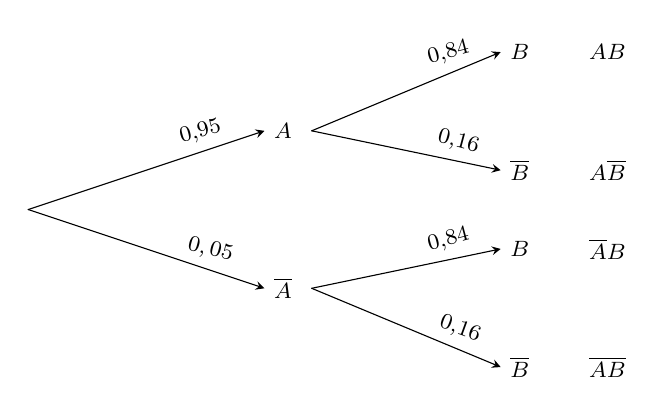
\begin{tikzpicture}[line join=round,line cap=round, font=\footnotesize,scale=1,>=stealth]
				\draw[-stealth](0,0)--(3,1)node[above, near end,,rotate=15]{$0{,}95$}node[right]{$A$};	
				\draw[-stealth](3.6,1)--(6,2)node[above, near end,,rotate=15]{$0{,}84$}node[right]{$B$};
				\draw(7,2)node[right]{$AB$};
				\draw[-stealth](3.6,1)--(6,0.5)node[above, near end,,rotate=-15]{$0{,}16$}node[right]{$\overline{B}$};
				\draw(7,0.5)node[right]{$A\overline{B}$};
				\draw[-stealth](0,0)--(3,-1)node[above, near end,,rotate=-15]{$0,05$}node[right]{$\overline{A}$};
				\draw[-stealth](3.6,-1)--(6,-0.5)node[above, near end,,rotate=15]{$0{,}84$}node[right]{$B$};
				\draw(7,-0.5)node[right]{$\overline{A}B$};
				\draw[-stealth](3.6,-1)--(6,-2)node[above, near end,,rotate=-20]{$0{,}16$}node[right]{$\overline{B}$};
				\draw(7,-2)node[right]{$\overline{A}\overline{B}$};
			\end{tikzpicture}	
		\end{center}
		Xác suất để có đúng một loại hạt lúa nảy mầm là $$\mathrm{P}\left(A \overline{B} \cup \overline{A} B\right)=\mathrm{P}\left(A\overline{B}\right)+\mathrm{P}\left(\overline{A} B\right) = 0{,}95 \cdot 0{,}16 +   0{,}05 \cdot 0{,}84= 0{,}194.$$
	}
\end{ex}

%C:\Users\hppp\Desktop\Toan\ChuyenDeGK-CK-cacTruong\1.SAULUOI2025\SpDuAn-A-Dot11\data\HKII\1-TN-DS-TLN-TL-THPT-QueSon-QuangNam-HKII-NH24-25.tex
\begin{ex}[Trích đề HKII 2024 - 2025 THPT Quế Sơn - Quảng Nam]%[Đề thi HK2 lớp 11 THPT Quế Sơn-Quảng Nam năm học 2024-2025]%[Vân Giang]%[1D9H2-4]
	Lớp 11A có $40$ học sinh, trong đó có $16$ học sinh giỏi Toán, $20$ học sinh giỏi Văn và $12$ học sinh giỏi cả hai môn đó. Chọn ngẫu nhiên một học sinh của lớp. Tính xác suất để chọn được học sinh giỏi ít nhất một trong hai môn Toán hoặc Văn.
	
	\loigiai {
		Gọi $A$ là biến cố \lq\lq Học sinh đó giỏi Toán\rq\rq.\\
		$B$ là biến cố \lq\lq Học sinh đó giỏi Văn\rq\rq.\\
		Khi đó 
		$AB$ là biến cố \lq\lq Học sinh đó giỏi cả Toán và Văn\rq\rq.\\
		$A\cup B$ là biến cố \lq\lq Học sinh đó giỏi ít nhất một trong hai môn Toán và Văn\rq\rq.\\
		Xác suất để chọn được học sinh giỏi ít nhất một trong hai môn Toán hoặc Văn là 
		$$\mathrm{P}(A \cup B)=\mathrm{P}(A)+\mathrm{P}(B)-\mathrm{P}(AB) =\dfrac{16}{40}+\dfrac{20}{40}-\dfrac{12}{40}=\dfrac{3}{5}.
		$$
	}
\end{ex}

%C:\Users\hppp\Desktop\Toan\ChuyenDeGK-CK-cacTruong\1.SAULUOI2025\SpDuAn-A-Dot12\data\HKII\1-TL-TN-DS-TLN-THPT-PhanBoiChau-BinhThuan-HKII-NH24-25.tex
\begin{ex}[Trích đề HKII 2024 - 2025 THPT Phan Bội Châu - Bình Thuận]%[1D9V2-3]%[Dự án đề kiểm tra Toán HKII NH24-25 - Đợt 12 - Hieu Phan]%[THPT Phan Bội Châu - Bình Thuận]
	Một hộp đựng $15$ tấm thẻ cùng loại được đánh số lần lượt từ $1$ đến $15$. Rút ngẫu nhiên ba thẻ. Tính xác suất để tổng ba số ghi trên ba thẻ lấy ra là một số chẵn.
	\loigiai{
		Gọi $\Omega$ là không gian mẫu, bao gồm tất cả các cách chọn ngẫu nhiên $3$ thẻ từ $15$ thẻ.\\
		Ta có $ n\left(\Omega\right)=\mathrm{C}_{15}^3=455$.\\
		Gọi $ A$ là biến cố "lấy ra được ba thẻ mang số chẵn".\\
		Gọi $ B$ là biến cố "lấy ra được hai thẻ mang số lẻ và một thẻ mang số chẵn".\\
		Ta có $ A,B$ là hai biến cố xung khắc.\\
		$\mathrm{P}(A)=\dfrac{\mathrm{C}_7^3}{\mathrm{C}_{15}^3}=\dfrac{35}{455}$.\\
		$\mathrm{P}(B)=\dfrac{\mathrm{C}_8^2\cdot \mathrm{C}_7^1}{\mathrm{C}_{15}^3}=\dfrac{196}{455}$.\\
		Vậy, xác suất để tổng ba số ghi trên ba thẻ lấy ra là một số chẵn là 
		$$\mathrm{P}(A\cup B)=\dfrac{35}{455}+\dfrac{196}{455}=\dfrac{231}{455}=\dfrac{33}{65}.$$}
\end{ex}

%C:\Users\hppp\Desktop\Toan\ChuyenDeGK-CK-cacTruong\1.SAULUOI2025\SpDuAn-A-Dot12\data\HKII\1-TN-DS-TLN-TL-THPT-NgoGiaTu-DakLak-GHKII-NH23-24.tex
\begin{ex}[Trích đề HKII 2024 - 2025 THPT Ngô Gia Tự - Daklak]%[1D9V2-4]%[Dự án đề kiểm tra Toán 11 HKII NH24-25- Mui Doan]%[THPT NGÔ GIA TỰ - Daklak]
	Chọn ngẫu nhiên $3$ số $a$, $b$, $c$ từ tập $T=\{1; 2; 3; \ldots.; 28\}$. Tính xác suất chọn được $3$ số thỏa mãn $a^2+b^2+c^2$ chia hết cho $5$.
	\loigiai{
		Gọi $A$ là tập hợp gồm các số chia hết cho $5$, ta có $n(A)=5$ \\
		Gọi $B$ là tập hợp gồm các số chia $5$ dư $1$ hoặc $4$, ta có $n(B)=11$.\\
		Gọi $C$ là tập hợp gồm các số chia $5$ dư $2$ hoặc $3$, ta có $n(C)=12$. \\
		Số phần tử của không gian mẫu là $\mathrm{C}_{28}^3=3\,276$.
		\begin{itemize}
			\item TH1: Chọn $3$ số thuộc $A$ có $\mathrm{C}_5^3=10$.
			\item TH2: Chọn $1$ số thuộc $A$, $1$ số thuộc $B$ và $1$ số thuộc $C$ có $\mathrm{C}_5^1\cdot\mathrm{C}_{11}^1\cdot\mathrm{C}_{12}^1=660$.
		\end{itemize}
		Gọi $D$ là biến cố được $3$ số $a$, $b$, $c$ thỏa mãn $a^2+b^2+c^2$ chia hết cho $5$.\\
		Ta có  $\mathrm{P}(D)=\dfrac{10+660}{3\,276}=\dfrac{335}{1\,638} \approx 0{,}2$.
	}
\end{ex}